% ============================================================
%  SCHOLA DOMESTICA — Magister Mathematica
%  Level 1 | Week 7 | Day 5
%  WEEK 7 REVIEW — Introduction to Addition
% ============================================================
\documentclass[12pt, letterpaper]{article}

\usepackage[top=1in, bottom=1in, left=1in, right=1in]{geometry}
\usepackage{fontenc}
\usepackage{inputenc}
\usepackage{lmodern}
\usepackage{microtype}
\usepackage{amsmath}
\usepackage{graphicx}
\usepackage{xcolor}
\usepackage{tikz}
\usepackage{array}
\usepackage{enumitem}
\usepackage{multicol}
\usepackage{mdframed}
\usepackage{fancyhdr}

\definecolor{scholared}{RGB}{160,30,30}
\definecolor{scholagold}{RGB}{180,140,40}
\definecolor{scholacream}{RGB}{253,248,235}
\definecolor{scholagreen}{RGB}{50,110,60}
\definecolor{scholablue}{RGB}{40,80,140}

\pagestyle{fancy}
\fancyhf{}
\renewcommand{\headrulewidth}{0.6pt}
\fancyhead[L]{\small\textcolor{scholared}{\textbf{Schola Domestica — Magister Mathematica}}}
\fancyhead[R]{\small\textcolor{scholared}{Level 1 · Week 7 · Day 5 (Review)}}
\fancyfoot[C]{\small\textcolor{gray}{— \thepage\ —}}

\newcommand{\answerline}{\underline{\hspace{2.5cm}}}
\newcommand{\biganswerline}{\underline{\hspace{4cm}}}
\newcommand{\numbox}{\fbox{\hspace{0.6cm}\vphantom{0}}}
\newcommand{\symbox}{\fbox{\hspace{0.7cm}}}

\newmdenv[
  backgroundcolor=white,
  linecolor=scholagold,
  linewidth=2pt,
  roundcorner=6pt,
  innertopmargin=8pt,
  innerbottommargin=8pt,
  innerleftmargin=10pt,
  innerrightmargin=10pt
]{scorebox}

\newmdenv[
  backgroundcolor=scholacream,
  linecolor=scholared,
  linewidth=1.5pt,
  roundcorner=6pt,
  innertopmargin=8pt,
  innerbottommargin=8pt,
  innerleftmargin=10pt,
  innerrightmargin=10pt
]{lessonbox}

\begin{document}

\begin{center}
  {\LARGE\textbf{\textcolor{scholared}{Week 7 Review}}}\\[4pt]
  {\Large\textcolor{scholagold}{\textit{Introduction to Addition}}}\\[6pt]
  {\small Name: \biganswerline \hspace{1cm} Date: \answerline}\\[4pt]
  {\small\textit{Work carefully. Check your answers by counting.}}
\end{center}

\vspace{4pt}
\noindent\textcolor{scholared}{\rule{\linewidth}{1.5pt}}
\vspace{4pt}

% ===== S1: PICTURE ADDITION =====
\noindent\textcolor{scholared}{\large\textbf{Section 1 — Picture Addition}} \hfill \textit{(4 points)}

\medskip\noindent\textit{Count each group and write the addition sentence.}

\bigskip
\noindent\textbf{1.}

\begin{tikzpicture}[baseline=-0.5ex]
  \foreach \i in {1,...,5}{\filldraw[scholablue](\i*0.4,0)circle(0.13cm);}
\end{tikzpicture}
\; $+$ \;

\begin{tikzpicture}[baseline=-0.5ex]
  \foreach \i in {1,...,3}{\filldraw[scholared](\i*0.4,0)circle(0.13cm);}
\end{tikzpicture}
\hspace{1cm}
\numbox \; $+$ \; \numbox \; $=$ \; \numbox

\bigskip
\noindent\textbf{2.}

\begin{tikzpicture}[baseline=-0.5ex]
  \foreach \i in {1,...,7}{\filldraw[scholagreen](\i*0.4,0)circle(0.13cm);}
\end{tikzpicture}
\; $+$ \;

\begin{tikzpicture}[baseline=-0.5ex]
  \foreach \i in {1,...,2}{\filldraw[scholagold](\i*0.4,0)circle(0.13cm);}
\end{tikzpicture}
\hspace{1cm}
\numbox \; $+$ \; \numbox \; $=$ \; \numbox

\bigskip
\noindent\textcolor{scholared}{\rule{\linewidth}{0.4pt}}

% ===== S2: ADDITION FACTS =====
\noindent\textcolor{scholared}{\large\textbf{Section 2 — Addition Facts}} \hfill \textit{(8 points)}

\bigskip
\begin{multicols}{4}
\noindent\textbf{3.} $6+2=$ \numbox\\[10pt]
\noindent\textbf{4.} $4+1=$ \numbox\\

\columnbreak
\noindent\textbf{5.} $3+0=$ \numbox\\[10pt]
\noindent\textbf{6.} $5+4=$ \numbox\\

\columnbreak
\noindent\textbf{7.} $7+1=$ \numbox\\[10pt]
\noindent\textbf{8.} $2+8=$ \numbox\\

\columnbreak
\noindent\textbf{9.} $0+9=$ \numbox\\[10pt]
\noindent\textbf{10.} $5+5=$ \numbox\\
\end{multicols}

\bigskip
\noindent\textcolor{scholared}{\rule{\linewidth}{0.4pt}}

% ===== S3: NUMBER LINE =====
\noindent\textcolor{scholared}{\large\textbf{Section 3 — Number Line Addition}} \hfill \textit{(2 points)}

\begin{center}
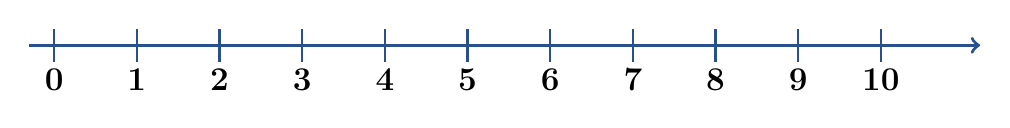
\begin{tikzpicture}[scale=1.05]
  \draw[very thick, scholablue, ->] (-0.3,0) -- (11.2,0);
  \foreach \n in {0,...,10} {
    \draw[thick, scholablue] (\n,0.2) -- (\n,-0.2);
    \node[below=5pt] at (\n,0) {\large\textbf{\n}};
  }
\end{tikzpicture}
\end{center}

\noindent\textbf{11.} Draw hops for $6+3$. Answer: \hfill \answerline \hspace{2cm}
\textbf{12.} Draw hops for $8+2$. Answer: \hfill \answerline

\bigskip
\noindent\textcolor{scholared}{\rule{\linewidth}{0.4pt}}

% ===== S4: WORD PROBLEMS =====
\noindent\textcolor{scholared}{\large\textbf{Section 4 — Word Problems}} \hfill \textit{(4 points)}

\bigskip
\noindent\textbf{13.} A vase has 6 white flowers and 3 yellow flowers. How many flowers? 

\medskip
\hspace{2em} \numbox \; $+$ \; \numbox \; $=$ \; \numbox

\bigskip
\noindent\textbf{14.} William reads 4 pages in the morning and 4 pages at night. How many pages?

\medskip
\hspace{2em} \numbox \; $+$ \; \numbox \; $=$ \; \numbox

\bigskip
\noindent\textcolor{scholared}{\rule{\linewidth}{0.4pt}}

% ===== S5: DRAW =====
\noindent\textcolor{scholared}{\large\textbf{Section 5 — Draw an Addition}} \hfill \textit{(2 points)}

\bigskip
\noindent\textbf{15.} Draw a picture to show $3 + 5 = 8$:

\begin{center}
\begin{tikzpicture}
  \draw[thick, scholagold] (0,0) rectangle (13, 2.5);
\end{tikzpicture}
\end{center}

\bigskip
\noindent\textcolor{scholared}{\rule{\linewidth}{1pt}}

\begin{scorebox}
\begin{center}
\large\textbf{Score: \answerline / 20} \hspace{2cm}
\textbf{Parent/Teacher Initial: \answerline}\\[6pt]
\small\textit{Mastery = 17/20 or above.}
\end{center}
\end{scorebox}

\end{document}
